\section{The Clausius Inequality}

Consider two heat engines, one a reversible (Carnot) engine and the other an irreversible heat engine. For purposes of developing the Clausius Inequality we assume that both engines are sized to accept the same amount of heat $Q_H$ from the thermal source. Thus since the irreversible engine must be less efficient than the Carnot engine, it must reject more heat $Q_{L,irrev}$ to the thermal sink than that rejected by the Carnot engine $Q_{L,rev}$ , as shown:
\begin{figure}[H]
  \centering
  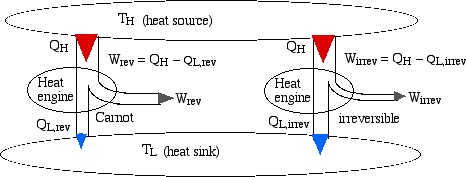
\includegraphics[width=.8\linewidth]{2engines}
  \caption{A reversible heat engine, producing more work than a comparable irreversible heat engine.}
  \label{fig:2engines}
\end{figure}

Consider first the reversible (Carnot) heat Engine. We saw in Chapter 5 that reversible heat transfer can only occur isothermally, thus the cyclic integral of the heat transfer divided by the temperature can be evaluated as follows:

\begin{equation}\label{eq:heatTransCycle}
  \oint \frac{\delta q}{T} = \int_H \frac{\delta q}{T} + \int_L \frac{\delta q}{T} = \frac{Q_H}{T_H} - \frac{Q_{L,rev}}{T_L}
\end{equation}

Recall from Chapter 5 that whenever we considered the efficiency of a reversible heat engine, we could replace the ratio of heat flows with the ratio of temperatures:
\begin{equation*}
  \frac{Q_H}{Q_L} = \frac{T_H}{T_L} \quad\rightarrow\quad \frac{Q_H}{T_H} = \frac{Q_{L}}{T_L}
\end{equation*}

From this, we can say that {\bf for reversible systems},
\begin{equation*}
  \oint \frac{\delta q}{T} = 0
\end{equation*}

Now, from Figure \ref{fig:2engines}, we see that $Q_H$ is the same for both engines, but $Q_{L,rev} < Q_{L, irrev}$.

For an irreversible engine, we can repeat our analysis from Equation \ref{eq:heatTransCycle}:
\begin{equation*}
  \oint \frac{\delta q}{T} = \int_H \frac{\delta q}{T} + \int_L \frac{\delta q}{T} = \frac{Q_H}{T_H} - \frac{Q_{L,irrev}}{T_L}
\end{equation*}

We can then subtract $\frac{Q_H}{T_H} - \frac{Q_{L,rev}}{T_L}$, since it is equal to 0:
\begin{equation*}
  \oint \frac{\delta q}{T} = \frac{Q_H}{T_H} - \frac{Q_{L,irrev}}{T_L} - \left(\frac{Q_H}{T_H} - \frac{Q_{L,rev}}{T_L}\right) =  \frac{Q_{L,rev} - Q_{L,irrev}}{T_L}
\end{equation*}

Finally, because $Q_{L,rev} < Q_{L, irrev}$, we can say:
\begin{equation}\label{eq:ClausiusInequality}
  \oint \frac{\delta q}{T} \le 0
\end{equation}

Equation \label{eq:ClausiusInequality} is known as the Clausius Inequality.

\section{Defining Entropy}
All properties (such as pressure, temperature, etc.) have a cyclic integral equal to zero, meaning that if we follow the change of the property through a full cycle, the total change will be zero.

For example, following the change of temperature through a cycle with $n$ processes:
\begin{align*}
  \oint dT &= \int_1^2 dT + \int_2^3 dT + ... + \int_{n-1}^n dT+ \int_n^1 dT\\
  \oint dT &= \left(T_2 - T_1\right) + \left(T_3 - T_2\right) + ... + \left(T_n - T_{n-1}\right) + \left(T_1 - T_n\right) = 0
\end{align*}

For reversible machines, since $\oint \frac{\delta q}{T} = 0$, we can define a property $S$, named {\bf entropy} such that:
\begin{equation} \label{eq:entropyDef}
  dS = \left.\frac{\delta q}{T}\right|_{rev}
\end{equation}
Integrating over a process at a temperature $T_0$ yields:
\begin{align*}
  \int dS &= \int \left.\frac{\delta q}{T}\right|_{rev} \\
  \Delta S &= \left.\frac{Q}{T_0}\right|_{rev}
\end{align*}

In other words, for reversible processes, entropy is increased through heat transfer into our control volume.  At higher temperatures, the entropy increase is lower than for low temperatures.

\subsection{Increase of Entropy for a Control Mass}

Consider an irreversible cycle in which process (1) -> (2) follows an irreversible path, and process (2) -> (1) a reversible path, as shown:

\begin{figure}[H]
  \centering
  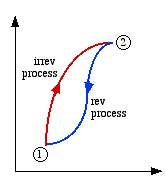
\includegraphics[width=.4\linewidth]{increase}
  \caption{A pair of processes between two points.  The process in red follows an irreversible path, and the process in blue follows the reversible path.}
  \label{fig:increase}
\end{figure}

Now, considering the Clausius inequality, we can state:
\begin{align*}
  \oint \frac{\delta q}{T} &= \left(\int_1^2 \frac{\delta q}{T}\right)_{irrev} +\left(\int_2^1 \frac{\delta q}{T}\right)_{rev} < 0\\
  \left(\int_1^2 \frac{\delta q}{T}\right)_{irrev} + \int_2^1 dS &= \left(\int_1^2 \frac{\delta q}{T}\right)_{irrev} + S_1 - S_2 < 0 \\
  \Delta S &= S_2 - S_1 > \int_1^2 \frac{\delta q}{T}
\end{align*}

If we limit our analysis to adiabatic processes ($\delta q =0$),
\begin{equation*}
  Q = 0 \quad\rightarrow\quad \redbox{\Delta S \ge 0}
\end{equation*}

Thus the entropy change of an adiabatic process is always greater than or equal to zero, where the equality applies to reversible processes. However not all processes are adiabatic. Nevertheless we can always enclose a system in a surrounding environment which is adiabatic, thus considering the total entropy change of both the system and surroundings we obtain:

\begin{figure}[H]
  \centering
  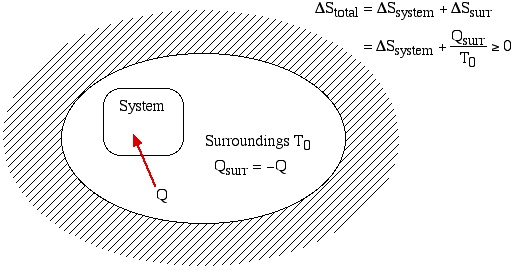
\includegraphics[width=.9\linewidth]{sgen_system}
  \caption{Heat transfer into a system from the surroundings.  Globally, entropy will either stay the same or increase.}
  \label{fig:sgen_system}
\end{figure}

Calculating the total entropy generated, $S_{gen}$:
\begin{align*}
  S_{gen} &= \Delta S_{total} = \Delta S_{system} + \frac{Q_{surr}}{T_0} \ge 0 \\
  \frac{S_{gen}}{m} = s_{gen} &= \Delta s_{system} + \frac{q_{surr}}{T_0} \ge 0
\end{align*}

\begin{quoteWithTitle}{Increase in Entropy Principle}
  For any process the total change in entropy of a system together with its enclosing adiabatic surroundings is always greater than or equal to zero.
\end{quoteWithTitle}

The total change of entropy is denoted $S_{gen}$ [kJ/K] or $s_{gen}$ [kJ/kg.K]).

\subsection{Increase of Entropy for a Control Volume}
We now consider the entropy generated during a steady flow process through a single-input/single-output control volume (CV) enclosed in an adiabatic surroundings as shown:%
\nopagebreak[4]%
\begin{figure}[H]
  \centering
  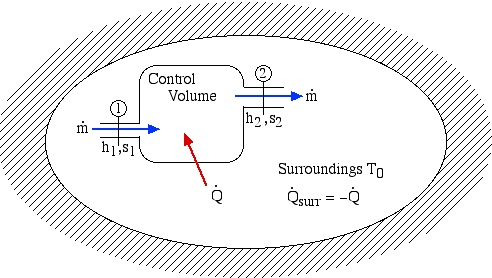
\includegraphics[width=.7\linewidth]{sgen_flow}
  \caption{Heat transfer into a control volume from the surroundings.  Globally, entropy will either stay the same or increase.}
  \label{fig:sgen_flow}
\end{figure}

\begin{equation*}
  \Delta\dot{S}_{total} = \cancelto{0}{\Delta\dot{S}_{CV}} + \Delta\dot{S}_{surr} \ge 0
\end{equation*}

Notice that for a steady flow system there can be no change of any of its property values with time, thus the rate of increase of entropy can only be associated with the surroundings. Notice also that at station (2) we are also dumping entropy from the control volume into the surroundings, and at station (1) we are sucking entropy out of the surroundings, leading to:
\begin{equation*}
  \dot{S}_{gen} = \Delta\dot{S}_{total} = \Delta\dot{S}_{surr} = \dot{m}(s_2-s_1) + \frac{\dot{Q}}{T_0} \ge 0
\end{equation*}

Dividing by $\dot{m}$:
\begin{equation*}
  \dot{s}_{gen} = \Delta{s}_{CV} = (s_2-s_1) + \frac{q}{T_0} \ge 0
\end{equation*}

Surprisingly the form of the specific entropy generated function $s_{gen}$ for a control volume is identical to that for a system.

For multiple-input, multiple-output control volumes under steady flow conditions, the entropy generated function is extended to:

\begin{equation*}
  \dot{S}_{gen} = \sum_e \dot{m}_es_e - \sum_i \dot{m}_is_i + \frac{\dot{Q}}{T_0} \ge 0
\end{equation*}

The summations are taken over all the exit ports (e) and inlet ports (i).

\subsection{Evaluating Entropy}
Recall from consideration of the Clausius Inequality that we defined entropy as follows:
\begin{equation*}
  \frac{\delta Q}{T} = dS
\end{equation*}

A very strange definition indeed, and difficult to comprehend. It is defined in differential format as the reversible heat transfer divided by the temperature. In an attempt to try and understand it we rewrite the definition as follows:

\begin{equation*}
  \delta Q = T dS \quad\rightarrow\quad Q = \int_{rev} T dS
\end{equation*}

This form may look familiar.  Recall our earlier definition of work:
\begin{equation*}
  \delta W = p dV \quad\rightarrow\quad W = \int_{rev} p dV
\end{equation*}

Thus it begins to make sense. Work done requires both a driving force (pressure $p$) and movement (volume change $dV$). We implicitly evaluated the work done for reversible processes - always neglecting friction or any other irreversibility.

Similarly we can state that heat transfer requires both a driving ``force'' (temperature $T$) and some equivalent form of "movement" (entropy change $dS$). Since temperature can be considered as represented by the vibration of the molecules, it is this transfer of vibrational energy that we define as entropy.

With both of the above equations in hand, we can write the differential form of the energy equation as follows:
\begin{align}
  \nonumber du &= \delta q - \delta w  \\
  \label{eq:Tds1} du &= T ds - p dv  &\rightarrow& \quad \redbox{Tds = du + pdv}
\end{align}
We can also rewrite Equation \ref{eq:Tds1} using enthalpy:
\begin{align}
  \nonumber dh = d(u + pv) &= du + pdv + vdp \\
  \label{eq:Tds2} du + pdv &= dh - vdp &\rightarrow& \quad \redbox{Tds = dh - vdp}
\end{align}

The major take-away from Equations \ref{eq:Tds1} and \ref{eq:Tds2} is as follows: given a process, which defines a path by which internal energy $u$ and specific volume $v$ change at a certain pressure $p$ and temperature $T$, we can calculate the change $ds$ along each step of the process.  This allows us to define a numerical value of entropy for every possible state.  These numerical values are given in the steam tables.

\subsection{Entropy for Ideal Gases}
For ideal gases, we can go further in our analysis.  Taking the ideal gas law ($pv = RT$) in conjunction with Equation \ref{eq:Tds1} allow us to write:
\begin{equation} \label{eq:idealEntropy1}
  ds  = \frac{du}{T}+ \frac{pdv}{T} \quad\rightarrow\quad ds = c_v \frac{dT}{T} + R\frac{dv}{v}
\end{equation}
Integrating \label{eq:idealEntropy1} (and assuming that $c_v$ is constant) results in:
\begin{align} 
  \nonumber  \int ds &= c_v \int \frac{dT}{T} + R \int \frac{dv}{v} \\
  \label{eq:idealEntropy2} s_2 - s_1 &= c_v \ln \left(\frac{T_2}{T_1}\right) + R \ln \left(\frac{v_2}{v_1}\right)
\end{align}

We can follow the same path with Equation \ref{eq:Tds2} as follows:
\begin{align}
  \nonumber ds  &= \frac{dh}{T}- \frac{vdp}{T} \quad \rightarrow\quad ds = c_p \frac{dT}{T} + R\frac{dv}{v} \\
  \nonumber  \int ds &= c_p \int \frac{dT}{T} - R \int \frac{dp}{p} \\
  \label{eq:idealEntropy3} s_2 - s_1 &= c_p \ln \left(\frac{T_2}{T_1}\right) - R \ln \left(\frac{p_2}{p_1}\right)
\end{align}

Equations \ref{eq:idealEntropy2} and \ref{eq:idealEntropy3} describe the change of entropy in an ideal gas.

\begin{quoteWithTitle}{Change of Entropy in an Ideal Gas}%
  \begin{equation*}
    s_2 - s_1 = c_v \ln \left(\frac{T_2}{T_1}\right) + R \ln \left(\frac{v_2}{v_1}\right) =
    c_p \ln \left(\frac{T_2}{T_1}\right) - R \ln \left(\frac{p_2}{p_1}\right)
  \end{equation*}
\end{quoteWithTitle}

\subsection{Entropy for Liquids and Solids}
For liquids and solids, we can use Equation \ref{eq:Tds1}, recognizing that $dv$ is zero for incompressible materials:

\begin{equation*}
  du = Tds - p\cancelto{0}{dv} \quad\rightarrow\quad ds = \frac{du}{T}
\end{equation*}

Assuming that the specific heat is a constant $c$, we can integrate as follows:
\begin{equation} \label{eq:entropyChangeIncompressible}
  \int ds = c\int\frac{dT}{T} \quad\rightarrow\quad s_2 - s_1 = c \ln \left(
 \frac{T_2}{T_1}\right)
\end{equation}

Therefore, entropy is defined purely by the temperature change for solids and liquids.

\section{Isentropic Processes}

The development of entropy as a property of a state allows us to consider processes that are isentropic.  For a process to be isentropic, it must satisfy two conditions:
\begin{itemize}
\item It must be adiabatic (no heat transfer)
\item It must be reversible (no friction, air resistance, mixing, etc.)
\end{itemize}

\subsection{Pure Substances}
For pure substances (steam, R134a, etc.), we evaluate an isentropic process by maintaining $\Delta s = 0$, or $s_2 = s_1$ and consulting the relevant tables.  This is exactly the same process as is used for isothermal, isobaric, or constant volume processes.

This is illustrated in the example below.
\begin{example}{Isentropic Compression of Steam}
  Steam is held in a piston at a pressure of $p_1$ = 10 bar and a temperature of \mbox{$T_1$ = 350°C}. It is then compressed isentropically to a pressure of $p_2$ = 12 bar.  Determine the new temperature of the steam.

  {\bf Solution:}

  Since we know two properties for steam, we can find entropy for state (1) from the superheated steam tables, which will also be the entropy for state (2).
  \begin{equation*}
    s_1 = 7.303 \frac{\rm kJ}{\rm kg K} \quad \rightarrow {\rm \bf isentropic} \rightarrow \quad s_2 = 7.303 \frac{\rm kJ}{\rm kg K}
    \end{equation*}
  Using the superheated steam tables for $p$ = 12 bar, we find the following:
  \begin{center}
    \def\arraystretch{1.5}
    \begin{tabular}{r|c|c|c|l}
      $s$ & 7.214 & $s_2$ = 7.303 & 7.379 & kJ/kgK \\ \cline{2-4}
      $T$ & 350 & $T_2$ = ? & 400 & °C
    \end{tabular}
    \def\arraystretch{1.0}
  \end{center}
  We can then use linear interpolation to find $T_2$:
  \begin{equation*}
    \frac{\Delta T_A}{\Delta T_B} = \frac{\Delta s_A}{\Delta s_B} \rightarrow\quad\rightarrow \frac{T_3 - 350}{400-350} = \frac{7.303 - 7.214}{7.379 - 7.214} = 0.54
  \end{equation*}
  Therefore, \redbox{T_2 = 377°C}.
\end{example}

\subsection{Ideal Gases}
For ideal gases, an isentropic process results in:
\begin{equation*}
  \cancelto{0}{s_2 - s_1} = c_v \ln \left(\frac{T_2}{T_1}\right) + R \ln \left(\frac{v_2}{v_1}\right)
\end{equation*}
Recalling our discussion of adiabatic processes back in Section \ref{sec:ch3_idealGasAdiabatic}, notice that this is equivalent to Equation \ref{eq:ch3_adiabaticTv}:
\begin{equation*}
  \ln \left(\frac{T_2}{T_1}\right) = -\frac{R}{c_v} \ln \left(\frac{v_2}{v_1}\right)
\end{equation*}

With this, we can finally see why Equations \ref{eq:ch3_adiabaticIdealGasTV}, \ref {eq:ch3_adiabaticIdealGaspV}, and \ref{eq:ch3_adiabaticIdealGaspT} are collectively known as the {\bf isentropic relations} for an ideal gas.

\begin{quoteWithTitle}{Isentropic Relations for Ideal Gases}%
  \begin{equation*}
    \frac{T_2}{T_1} = \left(\frac{v_2}{v_1}\right)^{-(\gamma -1)} \quad\quad\quad
    \frac{p_2}{p_1} = \left(\frac{v_1}{v_2}\right)^{\gamma} \quad\quad\quad
    \frac{p_2}{p_1} = \left(\frac{T_2}{T_1}\right)^{\frac{\gamma}{\gamma -1}}
  \end{equation*}
\end{quoteWithTitle}


\subsection{Solids/Liquids}

For incompressible matter, we refer to Equation \ref{eq:entropyChangeIncompressible}: 
\begin{equation*}
  \cancelto{0}{s_2 - s_1} = c \ln \left(\frac{T_2}{T_1}\right) \quad\rightarrow\quad T_2 = T_1
\end{equation*}

Therefore, an isentropic process is identical to an isothermal process for incompressible solids and liquids.

\section{Isentropic Efficiency}
One of the important applications of isentropic processes is in determining the efficiency of various adiabatic components. These include turbines, compressors and aircraft jet nozzles. Thus we have made the statement that steam turbines are designed to be adiabatic, and that any heat loss from the turbine will result in a reduction in output power, however only now can we make the statement that the ideal turbine is isentropic. This enables us to evaluate the {\bf isentropic efficiency} of these components.

There are two property diagrams involving entropy in common usage, the temperature-entropy ($T$-$s$) and enthalpy-entropy ($h$-$s$) "Mollier" diagrams. We will find that the $h$-$s$ diagram is extremely useful for evaluating adiabatic turbines and compressors, and complements the $p$-$h$ diagram which we used in Chapter 4 to evaluate entire steam power plants or refrigerator systems. The $h$-$s$ diagram for steam is presented below:
\nopagebreak[4]%
\begin{figure}[H]
  \centering
  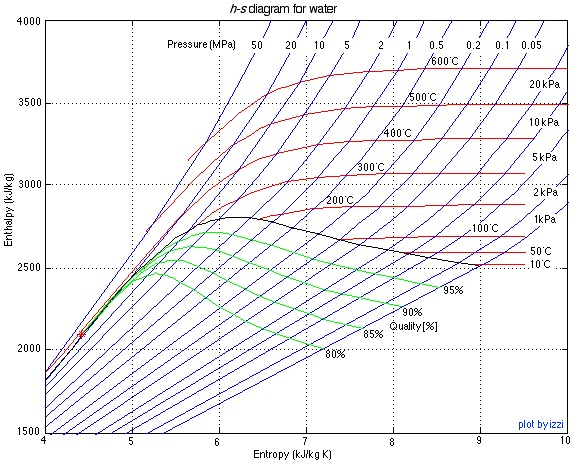
\includegraphics[width=.9\linewidth]{hs_water}
  \caption{The Mollier, or $h$-$s$ diagram, for water}
  \label{fig:hs_water}
\end{figure}
\subsection{Isentropic Efficiency of Turbines}
The important characteristic of the $h$-$s$ diagram is that the ideal adiabatic turbine can be conveniently plotted as a vertical line, allowing an intuitive visual appreciation of the turbine performance. We define the turbine adiabatic efficiency as follows:
\nopagebreak[4]%
\begin{figure}[H]
  \centering
  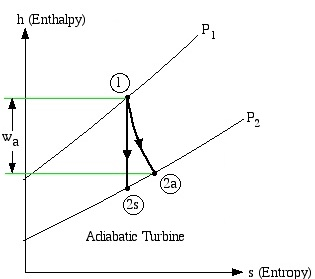
\includegraphics[width=.6\linewidth]{turbine_eff}
  \caption{An isentropic turbine process (1-2s) shown next to an actual turbine process (1-2a).}
  \label{fig:turbine_eff}
\end{figure}
\begin{equation} \label{eq:turbine_eff}
  \eta_T = \frac{\rm actual\ work}{\rm isentropic\ work} = \frac{w_a}{w_s} = \frac{h_1 - h_{2a}}{h_1 - h_{2s}}
\end{equation}

Notice that for the for the actual turbine there will always be an increase in entropy, which means that the turbine adiabatic efficiency will always be less than 100\%.

\begin{example}{Adiabatic Steam Turbine}
  Consider an adiabatic steam turbine having a turbine adiabatic efficiency $\eta_T$ = 80\%, operating under the conditions shown in the following diagram:
  
  \begin{center}
    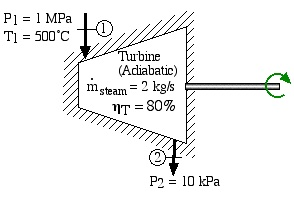
\includegraphics[width=0.7\linewidth]{isentropic_turbine_eff}
  \end{center}
  \begin{enumerate}[a)]
  \item Using steam tables, determine the enthalpy and entropy values at station (1) and station (2s) assuming that the turbine is isentropic. \answer{[$h_1$ = 3479 kJ/kg, $s_1$ = 7.764 kJ/kg.K; $h_{2s}$ = 2461 kJ/kg, $s_{2s}$ = $s_1$]}
  \item From the definition of turbine adiabatic efficiency, and given that $\eta_T$ = 80\%, determine the actual enthalpy and entropy values as well as the temperature at station (2a). \answer{[$h_{2a}$ = 2665 kJ/kg, $s_{2a}$ = 8.38 kJ/kg.K, $T_{2a}$ = 88°C]}
  \item Plot the actual and isentropic turbine processes (Stations (1)-(2a) and (1)-(2s)) on the enthalpy-entropy $h$-$s$ "Mollier" diagram, and indicate the actual turbine specific work ($w_a$) as well as the isentropic turbine specific work ($w_s$) on the diagram.
  \item Determine the actual power output of the turbine (kW). \answer{[1629 kW]}
  \end{enumerate}

  The $h$-$s$ diagram plot follows. Notice that we have indicated all the enthalpy and entropy values (which we determined from the steam tables) on the plot. This allows a check on the feasibility of our results.

  \begin{center}
    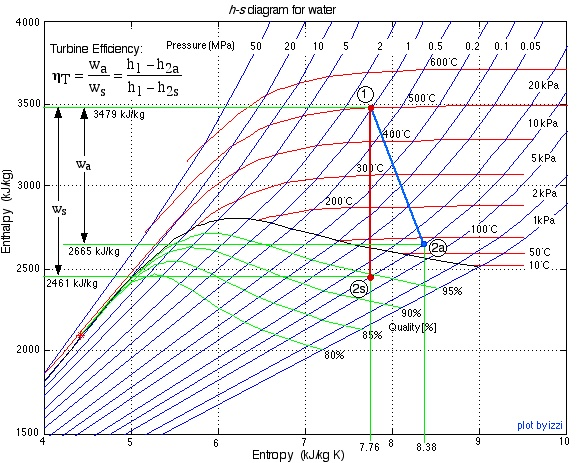
\includegraphics[width=0.8\linewidth]{hs_turbine}
  \end{center}
  
\end{example}

\subsection{Isentropic Efficiency of Compressors}

One of the interesting aspects of compressors is that they can be made more efficient by cooling. The reason why we still consider the adiabatic efficiency of compressors that are normally found in refrigeration, air-condition and heat pump systems is that it is considered to be impractical to cool them. Thus the ideal compressor (absorbing a minimum of power) is considered to be isentropic, and we define compressor adiabatic efficiency as follows:
\nopagebreak[4]%
\begin{figure}[H]
  \centering
  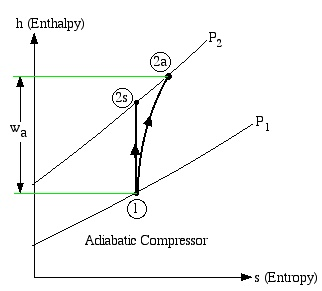
\includegraphics[width=.4\linewidth]{comp_eff}
  \caption{An isentropic compressor process (1-2s) shown next to an actual turbine process (1-2a).}
  \label{fig:turbine_eff}
\end{figure}

\begin{equation}\label{eq:comp_eff}
  \eta_C = \frac{\rm isentropic\ work}{\rm actual\ work} = \frac{w_s}{w_a} = \frac{h_{2s} - h_{1}}{h_{2a} - h_{1}}
\end{equation}

Notice that for the actual compressor there will always be an increase in entropy, leading to a compressor adiabatic efficiency which is less than 100\%.

\begin{example}{Adiabatic Compressor}
  Consider the R134a refrigerator compressor shown below.
  \begin{center}
    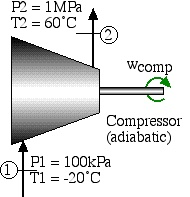
\includegraphics[width=0.3\linewidth]{comp_example}
  \end{center}

  \begin{enumerate}[a)]
  \item Carefully plot the actual and isentropic compression processes on the $h$-$s$ diagram and indicate the actual and isentropic specific work done to drive the compressor on the plot.
  \item Using R134a refrigerant tables determine the specific work required to drive the compressor \answer{[53.9 kJ/kg]}.
  \item Using R134a refrigerant tables determine the adiabatic efficiency of the compressor \answer{[$\eta_C$ = 92\%]}.
  \item Discuss these results and determine if this is a feasible compressor design.
  \end{enumerate}
  {\bf Solution:}

  Filling in information from tables for states 1 and 2:
  \begin{center}
    \def\arraystretch{1.5}
    \begin{tabular}{r|c|c|c|l}
       & State 1 & State 2 & State 2s & \\ \cline{2-4}
      $p$ & 100 & 1000 & 1000 & kPa \\ \cline{2-4}
      $T$ & -20 & 60 & ? & °C \\ \cline{2-4}
      $s$ & 0.972 & 0.985 & 0.972 & kJ/kgK \\ \cline{2-4}
      $h$ & 239.5 & 293.4 & ? & kJ/kg
    \end{tabular}
    \def\arraystretch{1.0}
  \end{center}
  
  \begin{center}
    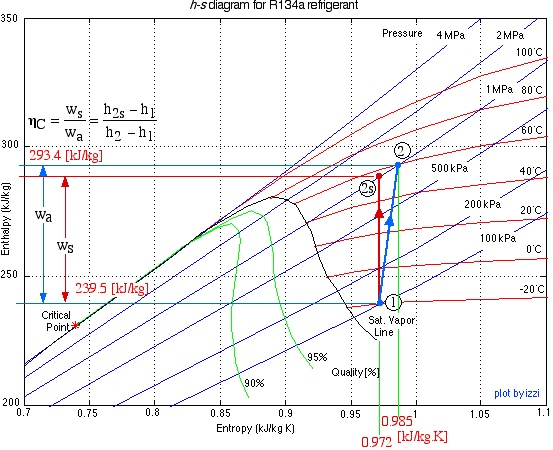
\includegraphics[width=0.75\linewidth]{hs_comp1}
  \end{center}
  
  \begin{center}
    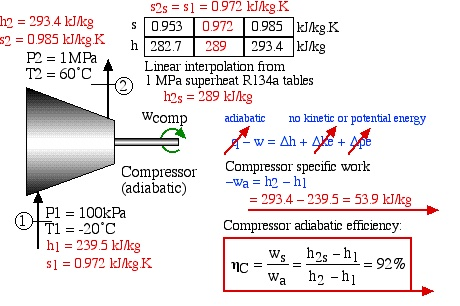
\includegraphics[width=0.6\linewidth]{comp1_eff}
  \end{center}
  
\end{example}

%--------------------------------------------------------------------
\section{Aircraft Engines}
%--------------------------------------------------------------------
There are many different forms and modifications of aircraft gas turbine engines, and in this course we discuss two variants - the ideal turbojet engine, and the gas turbine engine for usage in helicopters.

\begin{figure}[H]
  \centering
  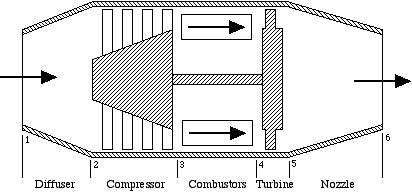
\includegraphics[width=.7\linewidth]{turbojet_schema}
  \caption{A simple diagram showing the five processes that make up a turbojet aircraft engine.}
  \label{fig:turbojet_schema}
\end{figure}

The ideal turbojet engine shown schematically in Figure \ref{fig:turbojet_schema} is comprised of the series connection of five components - diffuser, compressor, combustor, turbine, and nozzle. The analysis of the complete system, is best done in terms of the $h$-$s$ (enthalpy-entropy) diagram, which we will develop in class. Throughout the system we assume that the fluid is pure air, and the combustors are considered to be constant-pressure heat-addition devices. Notice that the sole purpose of the turbine is to drive the compressor, the nozzle providing the final kinetic energy increase to drive the aircraft.

The gas turbine engine for usage in helicopters is shown below:

\begin{figure}[H]
  \centering
  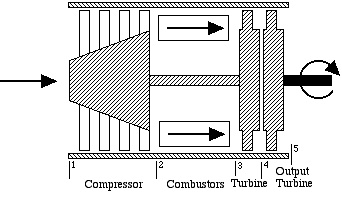
\includegraphics[width=.7\linewidth]{gasturb_schema}
  \caption{A simple diagram showing the five processes that make up a gas turbine helicopter engine.}
  \label{fig:gasturb_schema}
\end{figure}

In this case we see that there is no diffuser or nozzle, and that the turbine section has been replaced by two independent turbines - a "gas generator", or "gassifier" turbine to drive the compressor, and an output turbine to drive the helicopter blades. A typical gas turbine engine of this type is the General Electric T700 engine shown below, which is used in the Army Black Hawk helicopter.

\begin{figure}[H]
\centering
\begin{subfigure}{.5\textwidth}
  \centering
  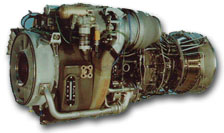
\includegraphics[width=.8\linewidth]{t700_baseline}
  \caption{Photograph of the GE T700 engine.}
  \label{fig:t700_baseline}
\end{subfigure}%
\begin{subfigure}{.5\textwidth}
  \centering
  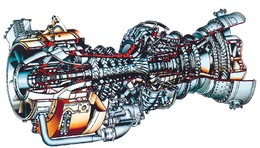
\includegraphics[width=.8\linewidth]{t700_section}
  \caption{Section view schematic of GE T700 engine.}
  \label{fig:t700_section}
\end{subfigure}
%\caption{}
%\label{fig:minimalHeatEnginePump}
\end{figure}

\begin{example}[label=ex:T700]{GE T700 Gas Turbine Engine}
  We wish to do an ideal thermodynamic analysis of the General Electric T700 gas turbine engine.
  \begin{center}
    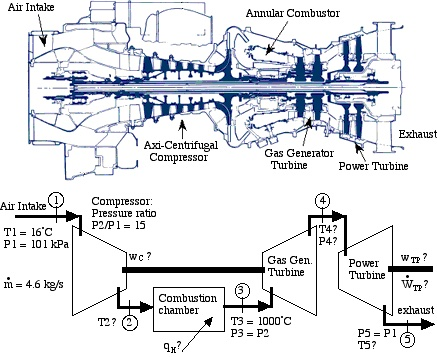
\includegraphics[width=.8\linewidth]{gas_turbine}
  \end{center}
  Notice that there are two turbines operating on independent output shafts. The High Pressure (first) turbine, named the Gas Generator Turbine, is directly connected by a shaft to the compressor. Its sole purpose is to drive the the axial/centrifugal compressor, thus the energy output of this turbine must equal the energy consumed by the compressor. The Low Pressure (second) turbine, named the Power Turbine, is connected via gearing to the helicopter rotor.

  {\bf Note:} Because of the large temperature variation throughout this problem we will need to consider the temperature dependence of the specific heat capacities of air. In the above schematic diagram we see that the temperature extremes of the system are 16°C - 1000°C (289 K - 1273 K), giving an average temperature of 781 K. From the table of Specific Heat Capacities of Air we see that at 800 K, $c_p$ = 1.099 [kJ/kgK] and the ratio of specific heat capacities $\gamma$ = 1.354, thus we use those values throughout this problem.
  
  Assume that the compressor and both turbines are isentropic, and that the combustion process occurs at constant pressure (isobaric). Using the information shown on the schematic diagram above, do the following:
  \begin{enumerate}[a)]
  \item  Sketch the entire process on an $h$-$s$ diagram, clearly showing the 5 stations on the diagram and the relevant isentropic and constant pressure lines.
  \item Determine the energy consumed by the compressor \answer{[$w_C$ = -328 kJ/kg]}, and the temperature at the outlet of the compressor \answer{[$T_2$ = 587 K]}.
  \item Determine the heat energy absorbed by the working gas in the combustion chamber \answer{[$q_H$ = 754 kJ/kg]}.
  \item Determine the temperature \answer{[$T_4$ = 975 K]} and the pressure \answer{[$p_4$ = 546 kPa]} at the outlet of the gas generator turbine.
  \item Determine the temperature \answer{[$T_5$ = 627 K]} and energy output of the power turbine \answer{[$w_{PT}$ = 382.5 kJ/kg]}.
  \item Given that the mass flow rate of the working gas through the system is 4.6 kg/s, determine the power output of the power turbine \answer{[1.76 MW]}.
  \end{enumerate}

  {\bf Solution:}
  information shown on the schematic diagram above, do the following:
  \begin{enumerate}[a)]
  \item  Sketch the entire process on an $h$-$s$ diagram, clearly showing the 5 stations on the diagram and the relevant isentropic and constant pressure lines.

    Unlike the case with a pure fluid such as steam, the $h$-$s$ diagram is not drawn to scale. Instead, is sketched in order to provide an intuitive graphical understanding of the problem.

    Furthermore, for an ideal gas the enthalpy is proportional to the temperature, hence the y-axis can be considered either an enthalpy or temperature axis. The various temperatures and pressures shown on this diagram are evaluated and plotted as we progress with the solution.

  \begin{center}
    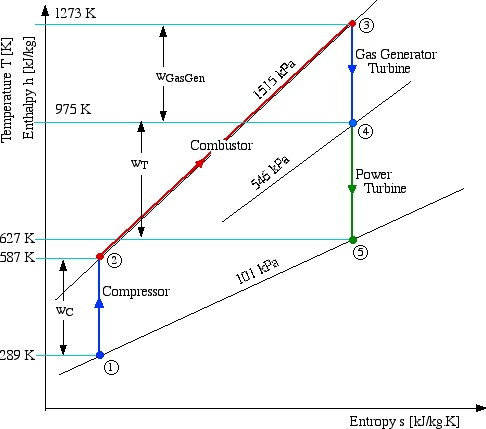
\includegraphics[width=.9\linewidth]{T700_h_s}
  \end{center}
      
   
\item Determine the energy consumed by the compressor, and the temperature at the outlet of the compressor.

  Ideally both the compressor and the turbine are isentropic devices, thus given the pressure ratio, in order to determine the temperature we consider the isentropic relations developed for an ideal gas.

  
  \begin{center}
    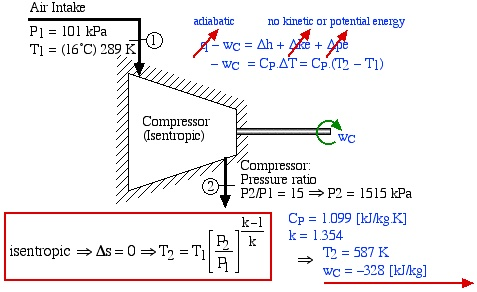
\includegraphics[width=.9\linewidth]{compressor}
  \end{center}
  
\item Determine the heat energy absorbed by the working gas in the combustion chamber.
  
  \begin{center}
    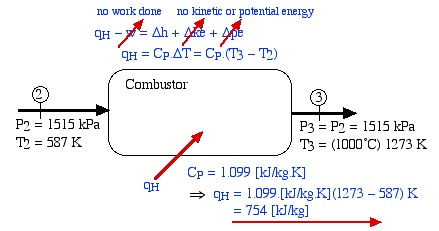
\includegraphics[width=.9\linewidth]{combustor}
  \end{center}
  
\item Determine the temperature and the pressure at the outlet of the gas generator turbine.

  Once more. since both turbines are isentropic, we use the pressure temperature relations developed for an isentropic process of an ideal gas.

  \begin{center}
    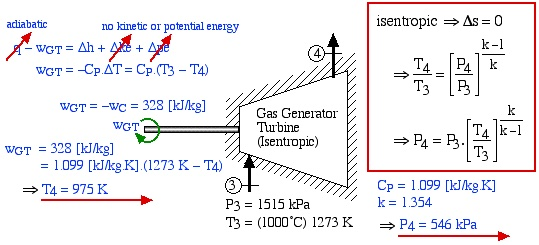
\includegraphics[width=.9\linewidth]{gasgen_turb}
  \end{center}
    
\item Determine the temperature and energy output of the power turbine.
  
  \begin{center}
    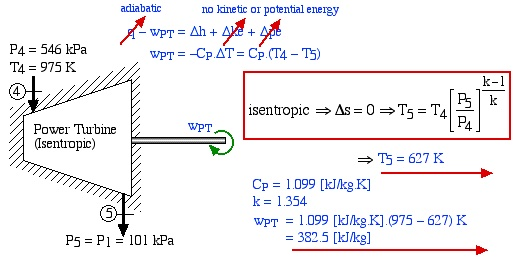
\includegraphics[width=.9\linewidth]{power_turb}
  \end{center}
\item Given that the mass flow rate of the working gas through the system is 4.6 kg/s, determine the power output of the power turbine.

  \begin{equation*}
    \dot{W}_{PT} = \dot{m} w_{PT} = 4.6 \frac{\rm kg}{\rm s} \cdot 382.5\frac{\rm kJ}{\rm kg} = 1.76\ {\rm MW}
  \end{equation*}
  \end{enumerate}

  Note that the actual power output of the T700 engine is around 1800 hp, which is significantly less than the above value ($\approx$ 2360 hp). This is because we have assumed that the compressor and both turbines are isentropic, which will never occur in practice. In a later problem, we will extend this exercise to consider a non-isentropic compressor and turbines.
\end{example}
\newpage
\begin{example}{T700 Proposed Turbojet Conversion}
  In Example \ref{ex:T700}, we did an ideal thermodynamic analysis of the General Electric T700 helicopter gas turbine engine. In theory, one could unclamp and remove the power turbine at the rear and replace it with a nozzle to form a turbojet engine.

Consider the schematic diagram of this conversion shown in the figure below:
  
  \begin{center}
    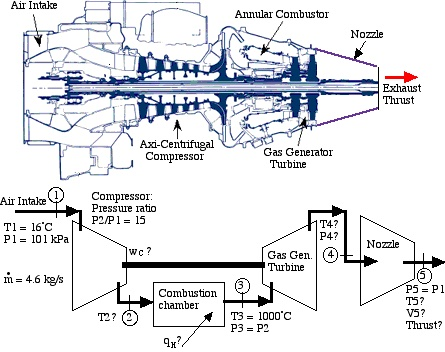
\includegraphics[width=.9\linewidth]{turbojet_T700}
  \end{center}

  Notice that the $h$-$s$ diagram has retained the same shape and characteristics as that in Example \ref{ex:T700}, with the only difference being that the change in enthalpy on the nozzle gives rise to a kinetic energy increase, rather than work output.

  \begin{center}
    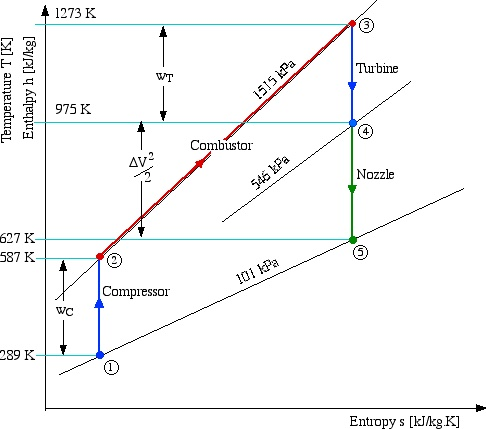
\includegraphics[width=.8\linewidth]{turbojet_h_s}
  \end{center}

  On replacing the power turbine with an isentropic jet nozzle, determine the temperature (T5) and exhaust velocity ($V_5$ - m/s). Given that the mass flow rate of the working gas through the system is 4.6 kg/s, determine the thrust force at the outlet of the nozzle (Thrust5 - lbf). [Note: 1 lbf (pound force) = 4.46 N]

  \begin{center}
    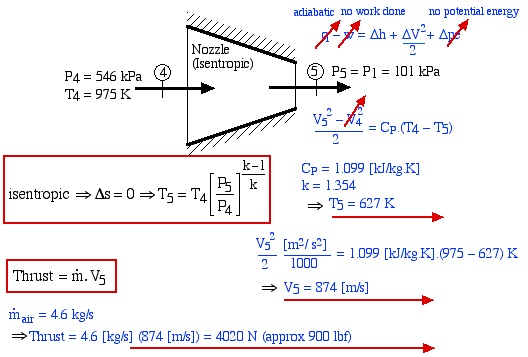
\includegraphics[width=.9\linewidth]{nozzle}
  \end{center}

\end{example}

\begin{example}{Flying at altitude}

  A theoretical jet engine is used to power a plane's flight at an altitude of 20 km and a speed of 200 m/s.  

  All that is known about the engine is that the compressor's pressure ratio is 18, and the turbine inlet temperature is 1250 K.

  Determine the thrust of the engine if the mass flow of air is 15 kg/s.  Find the thermal efficiency.
  \vspace{1em}
  
  {\bf Solution:}

  There are 6 total states that we need to determine \answer{[Answers using CoolProp]}:
  \begin{itemize}
  \item Atmosphere (a) - pressure and temperature at 20 km, with a velocity of 200 m/s \answer{[5474 Pa, 216.65 K]}
  \item Post-diffuser (1) - the diffuser will convert all of the kinetic energy of the air into enthalpy.  We will assume this is isentropic.  Kinetic energy is typically $KE = 1/2 m V^2$, but we tend to work in mass-specific units, so instead, we will find $ke = 1/2 V^2$.  This is in units of J/kg, so remember to convert to kJ/kg! \answer{[$h_1=$ 362.9 kJ/kg, $p_1$ = 7446 Pa]}
  \item Post-compressor, ideal (2s) - the compressor has a pressure ratio of 18.  We will assume isentropic for this state. \answer{[$h_{2s}$=668 kJ/kg]}
  \item Post-compressor, actual (2) - we will use the isentropic efficiency of a compressor (around 80-85 percent, we will use 82\%) to find the new enthalpy of this state, while assuming that the pressure remains the same. \answer{[$h_{2}$=735 kJ/kg]}
  \item Post-combustion (3) - we know the turbine inlet temperature, and will assume that the pressure remains the same from state 2. \answer{[$h_{3}$=1463 kJ/kg]}
  \item Post-turbine (4, 4s) - the total amount of work from the turbine ($h_4-h_3$) should be equal to the amount of work from the compressor ($h_2-h_1$).  This is not enough to determine a state by itself.  We assume that the pressure is constant between states 4 and 4s, and use the isentropic efficiency of a turbine (around 85-90 percent, we will use 91\%) to determine the enthalpy at state 4s.  The entropy is known there (same as $s_3$), so we can determine the pressure at state 4s, at which point all information is known for state 4. \answer{[$h_{4}$= 1091 kJ/kg, $h_{4s}$ = 1055 kJ/kg]}
  \item Post-nozzle (5) - we set the pressure back to atmospheric and assume that the nozzle operates isentropically.  The difference in energy ($h_5-h_4$) will be converted back to kinetic energy.  Remember to convert from kJ/kg to J/kg! \answer{[$h_{5}$=699 kJ/kg]}
  \end{itemize}

  Once we have all the states, we need to determine the thrust and the thermal efficiency:
  \begin{itemize}
  \item Thrust - $T = \dot{m}(V_e - V_i)$

    Once we have both the inlet and outlet velocity, this is relatively trivial.
    \answer{[Thrust=10.3 kN]}
  \item Thermal efficiency - $\eta_{th} = \left(ke_{\rm nozzle} - ke_{\rm diffuser}\right)/q_{\rm combustor}$

    We care about the thrust, which is in units of Newtons.  We are putting in energy as heat into the combustor, which is in units of kJ/kg. However, to find efficiency, we need to have consistent units between the two values.  The easiest thing to do is to find the kinetic energy converted within the nozzle and diffuser (since we already have the enthaply values).

    We can rewrite this as:
    \begin{equation}
      \eta_{th} = \frac{(h_1-h_a) - (h_4-h_5)}{(h_3-h_2)}
    \end{equation}
    \answer{[$\eta_{th}$ = 0.51]}
  \end{itemize}
  
  \vspace{1em}
  {\bf Important notes:}
  \begin{itemize}
  \item We should find the enthalpy at each state at a minimum.  If we are using CoolProp, we need the enthalpy and entropy at each state, at a minimum.  We can avoid finding the actual entropy if we are using the ideal gas assumption, unless we want to plot the cycle on the $h$-$s$ diagram.
  \item Whichever path we choose (ideal gas vs. CoolProp), we can write a code in Colab to find our states and efficiency.  If you use the ideal gas law, you can actually use Excel instead.  Be sure to choose good values for air properties!
  \item Pressure ratio is a ratio of pressures (unlike the compression ratio from Chapter 3, which was a ratio of volumes).
  \end{itemize}

  

  
\end{example}
\begin{homework}
  \question Consider the adiabatic steam turbine shown below.
  \begin{center}
    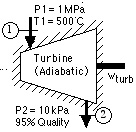
\includegraphics[width=0.3\textwidth]{steamTurb}
  \end{center}
  \begin{questionparts}
  \item Carefully plot the turbine process on the $h$-$s$ diagram and indicate the turbine work done on the plot.
  \item Using steam tables determine the specific work output of the turbine \answer{[1015 kJ/kg]}.
  \item Using steam tables determine the entropy generated by this process. \answer{[0.01 kJ/kg.K]}.
  \item Discuss these results and determine if this is a feasible turbine design.
  \end{questionparts}

  \question Adiabatic Evaluation of a R134a Compressor
  A young engineer was assigned to evaluate the compressor of a proposed R-134a refrigeration system shown below, and assumed it to be adiabatic.
  \begin{questionparts}
  \item Under this assumption, and ignoring kinetic and potential energy effects, determine the specific work input to the compressor \answer{[48.3 kJ/kg]}.
  \item His supervisor checked the results and told him that his assumption was incorrect and not physically feasible. On the $h$-$s$ diagram for R134a, draw the actual compression process (as assumed) as well as the equivalent isentropic compression process.
  \item Using the $h$-$s$ diagram, as well as relevant data evaluated at the inlet and outlet of the compressor, explain how she arrived at that conclusion.
  \end{questionparts}
  \newpage
  \question Previously, we provided a problem concerning a home refrigerator, and examining it's performance before and after adding an internal heat exchanger.
  \begin{center}
    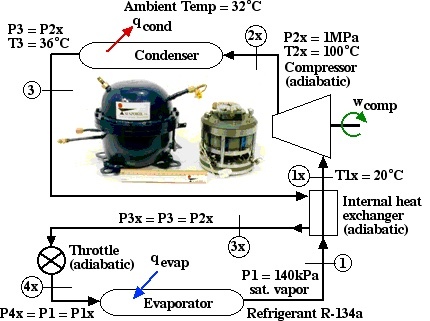
\includegraphics[width=0.5\textwidth]{ch4_HW_refrigHX}
  \end{center}
  \begin{questionparts}
  \item Plot the actual and the isentropic compressor processes on the enthalpy-entropy ($h$-$s$) diagram for both cases: with and without the internal heat exchanger.
  \item Using the R134a tables determine the actual compressor adiabatic efficiency ($\eta_C$) for both cases \answer{[75\%, 76\%]}
  \end{questionparts}

  \question A compressor is used to drive R134a through a heat pump.  R134a enters the compressor at a pressure $p_1$ = 400 kPa and a temperature $T_1$ = 40°C and leaves at a pressure $p_2$ = 1.6 MPa.  For the actual compressor, the exit tempearture is $T_2$ = 100°C.

  \begin{questionparts}
  \item Carefully plot the actual and isentropic compression processes on the $h$-$s$ diagram and indicate the actual and isentropic specific work done to drive the compressor on the plot.
  \item Using R134a refrigerant tables, determine the specific work required to drive the compressor \answer{[43.5 kJ/kg]}.
  \item Using R134a refrigerant tables, determine the adiabatic efficiency of the compressor \answer{[$\eta_C$ = 78\%]}.
  \item Discuss these results and determine if this is a feasible compressor design.
  \end{questionparts}
  \newpage
  \question In Example \ref{ex:T700} we did an ideal thermodynamic analysis of the General Electric T700 helicopter gas turbine engine, shown in the following schematic diagram:
  \begin{center}
    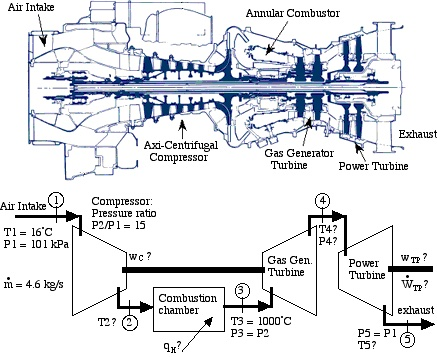
\includegraphics[width=.8\linewidth]{gas_turbine}
  \end{center}

  Notice again that there are two turbines operating on independent output shafts. The High Pressure (first) turbine, named the Gas Generator turbine, is directly connected by a shaft to the compressor. Its sole purpose is to drive the the compressor, thus the energy output of this turbine must equal the energy consumed by the compressor. The Low Pressure (second) turbine, named the Power turbine, is connected via gearing to the helicopter rotor.

  In Example \ref{ex:T700} we assumed that the compressor and both turbines were isentropic. In this exercise we wish to extend the analysis to non-isentropic compressor and turbines.

  Assume that the compressor adiabatic efficiency $\eta_C$ = 88\%, and that each turbine has an adiabatic efficiency $\eta_T$ = 86\%.

  \begin{questionparts}
  \item Sketch the entire process on an $h$-$s$ diagram, clearly showing the 5 stations on the diagram and the relevant isentropic and constant pressure lines. Indicate the relevant actual and isentropic work values on the sketch.
  \item Determine the actual energy consumed by the compressor \answer{[$w_{C,act}$ = 373 kJ/kg]}, and the actual temperature at the outlet of the compressor \answer{[$T_{2a}$ = 628K]}.
  \item Determine the heat energy absorbed by the working gas in the combustion chamber \answer{[$q_H$ = 709 kJ/kg]}.
  \item Determine the actual temperature [$T_{4a}$ = 934K] and the pressure [$P_4$ = 366 kPa] at the outlet of the gas generator turbine.
  \item Determine the actual temperature [$T_{5a}$] and energy output of the power turbine [$w_{PT,act}$ = 252 kJ/kg].
  \item Given that the mass flow rate of the working gas through the system is 4.6 kg/s, determine the actual power output of the power turbine \answer{[1161 kW]}.
  \item Determine the thermal efficiency ($\eta_{th}$) of the T700 gas turbine. Compare this value to the equivalent reversible thermal efficiency and discuss your results.
  \end{questionparts}

\end{homework}


